%% Public domain image from
%% http://www.public-domain-image.com/objects/computer-chips/slides/six-computers-chips-circuits.html
\renewcommand\chapterillustration{OGL_light/chapterImage}



\chapter{조명과 재질}

\index{조명}\index{lighting}
\index{재질}\index{material}

컴퓨터 그래픽스의 최종 결과는 시각 정보이다. 시각 정보는 우리의 눈을 통해 입력된다. 
눈이 인지하는 신호는 전자기파이며, 우리가 인지할 수 있는 영역의 전자기파를 가시광선(可視光線)이라 부른다.
이 가시광선을 일상적으로 `빛'이라 부른다. 빛은 시각정보를 생성하는 데에 있어 필수적인 요소이다.
같은 빛이라고 모든 물체가 같은 색으로 보이지는 않는다. 물체는 저마다의 `재질(材質,material)' 특성에 따라
서로 다른 방식으로 빛을 반사하여 다른 색상을 갖게 된다. 이 장에서는 이러한 현상을 실시간 그래픽스
환경에서 표현할 수 있는 이론적 배경과 실제 구현 방법을 이해하여 보자.

\section{조명과 음영}

음영(陰影) 계산, 혹은 셰이딩(shading)은 어떤 물체의 표면에서 어두운 부분과 밝은 부분을 서로 다른 밝기로 그려내는 것이다. 어떤 구를 그렸는데 그림 \ref{fig:OGL_light:shading}의 왼쪽과 같이 모든 면이 동일한 색으로 그리면 입체감이 없다. 구는 그림 \ref{fig:OGL_light:shading}의 오른쪽처럼 그려져야 한다.\index{음영}\index{shading}

\begin{figure}[h!]
  \centering
    
\includegraphics[height=4cm]{OGL_light/shading.png}
    \caption{음영의 효과: (왼쪽) 음영이 없는 렌더링 (오른쪽) 음영이 적용된 렌더링}
    \label{fig:OGL_light:shading}
\end{figure}

어떻게 하면 오른쪽 그림과 같은 입체적 느낌의 음영을 생성할 수 있는지가 이번 절의 주제이다. 왼쪽의 그림은 표면의 모든 지점이 동일한 색을 가지고 있는 것이고, 오른쪽 그림은 서로 다른 색을 가지고 있다. 색은 앞서 살펴본 것과 같이 눈에 의해 감지되는 전자기파, 즉 빛이다. 따라서 각각의 지점은 서로 다른 빛을 우리 눈에 보내고 있는 것이다.

구는 동일한 재질로 이루어졌지만, 조명과 물체의 상호작용이 동일한 재질의 구면 각각에서 서로 다른 빛을 눈에 보내도록 하는 것이다. 
이러한 상호작용에서 고려해야 하는 것들은 광원, 재질의 속성, 관찰자의 위치, 표면의 방향 등이 있다.

\subsection{지역조명(local illumination)과 전역조명(global illumination)}
\index{조명!지역조명}\index{조명!전역조명}
\index{지역조명}\index{전역조명}

색은 곧 감지된 빛이다. 빛은 광원에서 나온다. 광원을 출발한 빛이 물체에 닿으면 일부는 반사되고 일부는 흡수된다. 반사된 빛은 또 다시 다른 물체에 닿아 반사, 흡수를 반복한다. 이러한 과정은 무한히 반복되며, 눈에 도달한 빛은 그쪽 방향으로의 색을 결정하게 된다.


\begin{figure}[h!]
  \centering
    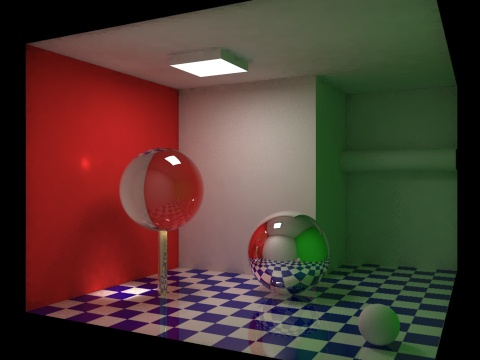
\includegraphics[height=6cm]{OGL_light/global_illumination.jpg}
    \caption{전역조명을 이용한 렌더링 결과}
    \label{fig:OGL_light:global_illumination}
\end{figure}

\begin{figure}[h!]
  \centering
    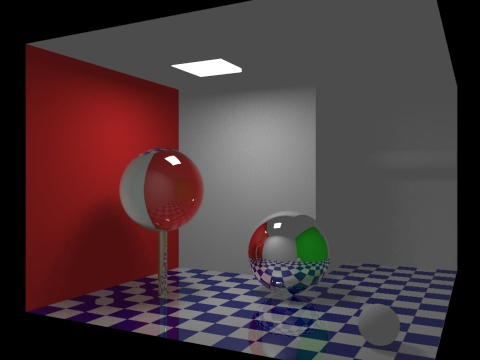
\includegraphics[height=6cm]{OGL_light/local_illumination.jpg}
    \caption{지역조명을 이용한 렌더링 결과}
    \label{fig:OGL_light:local_illumination}
\end{figure}

이러한 빛의 반사를 흉내내어 장면(scene) 안에 존재하는 모든 물체를 고려하여 빛의 반사를 계산하여 각 지점의 밝기와 색상을 계산하는 방식을 전역조명(global illumination)이라고 한다. 이 방법은 매우 사실적인 렌더링 결과를 얻을 수 있지만 계산량이 너무 커서 실시간 렌더링 환경에는 적합하지 않다.
어떤 빛이 물체에 닿아 반사된 빛까지 새로이 광원의 역할을 수행하는 것이 전역조명이라고 하면, 지역조명(local illumination) 모델은 렌더링하려는 
물체 외에는 어떤 다른 객체도 고려하지 않고 빛과 렌더링하는 물체 둘만의 관계를 이용하여 음영을 결정하는 방식이다. 


지역조명 모델은 물체 상호간의 빛 가림 등을 고려하지 않기 때문에 물체의 그림자 영역에 다른 물체가 들어가도 그림자가 지지 않고 밝게 렌더링 된다. 
이러한 이유로 원래의 지역조명은 그림자 등이 생길 수가 없다.
하지만 전역조명과 같이 사실적인 느낌을 주기 위해 빛의 굴절, 반사, 그림자 등을 텍스처 등을 활용하여 그려 넣을 수는 있다.
지역조명 모델에서 이러한 효과를 흉내낸다 하더라도 다른 객체에 반사된 빛에 의한 효과는 무시하기 전역조명에 비해서는
사실감이 떨어진다.
사실성을 포기한 대신에 지역조명은 매우 빠른 계산이 가능하다. 
따라서 게임이나 가상현실과 같은 실시간 응용에서는 각각의 표면이 조명과 어떤 관계에 놓여있는지만 고려하는 지역조명(local illumination)을 일반적으로 사용한다.


그림 \ref{fig:OGL_light:global_illumination}은 전역조명 기법을 이용하여 장면을 렌더링 한 결과이다. 이와 달리
그림 \ref{fig:OGL_light:local_illumination}은 지역조명을 이용하여 음영을 결정하고, 
텍스처 기술등을 활용하여 그림자, 굴절효과, 반사 등을 추가한 결과이다.
그림에서 볼 수 있는 바와 같이 지역조명에 비해 전역조명 모델이 훨씬 더 사실적인 결과를 보인다.

\subsection{광원 모델}
\index{광원}\index{light source}

일반적인 광원(光源, light source)은 다루기가 쉽지 않다. 하나의 광원은 일정한 면적이나 체적을 가지기 때문에 이 광원에서 나온 빛들을 적분해야 한다.
실제 실시간 렌더링에서는 광원을 하나의 점이나 방향으로 보는 단순화된 모델을 사용한다. 사용되는 광원은 다음과 같은 것들이 있다.

\begin{center}
    \begin{tabular}{ |l| p{12cm} |}
    \hline
    {\small \sf \bf 광원 종류} & {\small \sf \bf 특징} \\ \hline
    {\small \sf 점광원} & {\small \sf 광원의 위치와 색으로 결정. 전방향(omnidirection)으로 빛 진행.}\\ \hline
    {\small \sf 집중광원 } & {\small \sf 점광원에서 일부 입체각으로 빛을 제한.}\\ \hline
    {\small \sf 방향광원 } & {\small \sf 특정한 위치가 아니라 방향에 광원 존재.} \\ \hline
    {\small \sf 주변광원 } & {\small \sf 모든 곳에 동일하게 가해지는 빛.}\\ \hline
    \end{tabular}
\end{center}

\subsection{지역 조명 모델 - 퐁(Phong) 모델}\index{퐁 모델}\index{Phong model}

부드러운 면은 거울면과 같이 입사된 빛을 특정 반사 방향으로 집중적으로 보낸다. 이를 정반사(specular reflection)이라 한다. 
반면 거친 면은 미세면을 관찰하면 다양한 방향의 조각면들로 구성되어 있어 한쪽 방향이 아니라 반구형으로 여러 방향에 골고루 빛을 보낼 수 있다.
 이러한 반사를 난반사(diffuse reflection)이라고 한다. 실제 반사는 이러한 표면의 특성에 따라 매우 다양한 반사모델이 가능한데, 
단순화된 모델은 물체 표면의 반사를 이 두 반사의 조합으로 보고 각각 모델링하는 것이다. 대표적인 모델이 바로 퐁(Phong) 모델이다. 
이 반사 모델은 OpenGL이나 DirectX에서 기본적으로 사용되는 모델이다. 
퐁 모델은 물체의 정반사와 난반사 특성을 모두 표현할 수 있는 간단하고 빠른 모델이다. 이 모델에서는 다음과 같은 세 종류의 반사 요소가 있다.

\begin{itemize}
\item 난반사 (diffuse reflection)
\item 정반사 (specular reflection)
\item 주변광 반사 (ambient reflection)
\end{itemize}

이 반사의 정도를 계산하기 위해서는 다음과 같은 정보가 필요하다.

\begin{itemize}
\item 광원으로 향하는 벡터 $\mathbf L$
\item 카메라(시점)을 향하는 벡터 $\mathbf E$
\item 법선 벡터 $\mathbf N$
\item 이상적인 반사 방향 $\mathbf R$
\end{itemize}

이러한 정보가 가지는 의미가 그림 \ref{fig:OGL_light:lightingVectors}에 나타나 있다.

\begin{figure}[h!]
  \centering
    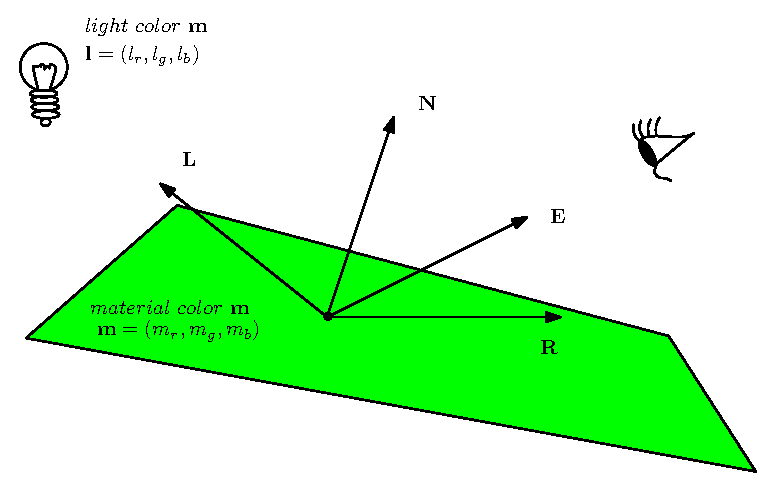
\includegraphics[height=6cm]{OGL_light/lightingVectors.eps}
    \caption{퐁(Phong) 모델에서 사용되는 방향 벡터들}
    \label{fig:OGL_light:lightingVectors}
\end{figure}

\index{Phong model}\index{퐁모델}
퐁 모델은 난반사, 정반사, 주변광을 각각 독립적으로 계산하여 합성한다. 각각의 반사 요소에 따라 결정해야 하는 것은 눈을 향해 오는 빛의 강도(intensity)와 색상이다. 
어떤 광원에서 나오는 빛의 색상이 $(l_r, l_g, l_b)$라고 하고, 물체의 재질 색상이 $(m_r, m_g, m_b)$라고 하자. 
빛의 색상은 이 빛이 눈에 감지되었을 때 우리가 느끼는 색이라고 할 수 있다. 그러면 물체의 재질 색상은 무엇일가? 예를 들어 빨간 색을 가진 물체의 
재질 색상 (1.0, 0.0, 0.0)은 무슨 의미일까? 이것은 도착하는 빛의 RGB 3 개 채널에서 R 채널의 빛을 100\% 반사한다는 것을 의미한다. 
따라서 반사되는 빛의 색상은 다음과 같다.

$$(l_r m_r, l_g m_g, l_b m_b)$$

빛의 색을 표현하는 3차원 벡터를 $\mathbf l$이라고 하고 물체의 재질 색을 3차원 벡터  $\mathbf m$이라고 하면 이 색상 값 $\mathbf c$는
벡터 각 차원별 성분의 곱을 의미하는 연산자 $\otimes$를 사용하여 간단히 다음과 같이 표현한다.

$$\mathbf c = \mathbf l \otimes \mathbf m = (l_r m_r, l_g m_g, l_b m_b) $$

이 계산은 눈에 감지되는 빛의 색상을 결정한다. 같은 색상이라도 밝고 어두운 곳이 있는데, 이러한 음영을 고려해야 입체적인 물체로 보이게 된다.
이러한 음영은 광강도(光强度, light intensity)에 의해 결정되는데, 이 광강도의 값은 스칼라(scalar) 값으로 $I$로 표현한다.
그러면 실제로 눈에 보이는 색은 광원과 재질에 의해 결정되는 색상 $\mathbf c$와 광강도 $I$에 의해 다음과 같이 결정된다.
\index{광강도}\index{light intensity}

$$\kappa = I \mathbf c$$

앞서 설명한 바와 같이 퐁 모델은 각각의 반사 요소를 모두 따로 계산한다. 난반사 요소와 관련된 값에는 아래첨자 d를 붙이고, 정반사에는 s, 주변광 반사에는 a를 붙이면 눈에 관측되는 색상은 다음 식 \ref{eq:PhongModel1}과 같다.

\begin{eqnarray}
\label{eq:PhongModel1}
\kappa & = & I_a \mathbf c_a + I_d \mathbf c_d + I_s \mathbf c_s
\end{eqnarray}

이때, 주변광의 광강도는 상수 값을 가지므로 $I_a$는 1로 설정할 수 있다. 따라서 식 \ref{eq:PhongModel1}은 다음 식 \ref{eq:PhongModel2}로 바꿀 수 있다.

\begin{eqnarray}
\label{eq:PhongModel2}
\kappa  =  \mathbf l_a \otimes \mathbf m_a + I_d \mathbf l_d \otimes \mathbf m_d + I_s \mathbf l_s \otimes \mathbf m_s
\end{eqnarray}

\section{퐁 모델 광강도(intensity)의 계산}

퐁 모델에서 우리가 계산해야 하는 광강도는 난반사 광강도 $I_d$와 정반사 광강도  $I_s$이다. 
이 가운데 우선 난반사 광강도를 먼저 구해 보자.


우리가 가정하는 난반사는 완벽한 난반사로 모든 방향에 동등하게 빛이 퍼진다. 따라서 눈이 어디에 있는지 동일한 색상 관찰이 이루어진다. 따라서 난반사는 눈의 움직임에 따라 변하는 하일라이트(highlight)는 표현하지 못하며, 색을 칠하려고 하는 한 지점에 대해 어디서 쳐다 보든지 동일한 밝기 정도를 결정한다. 이 밝기는 얼마나 많은 에너지(빛)가 해당 지점에 떨어지는지에 달려 있다. 이러한 개념은 그림 \ref{fig:OGL_light:diffuseConcept}에서 확인할 수 있다. 빛이 처음에 $I_{light}$의 강도로 표면에 떨어진다. 이때 
입사하는 각도에 수직으로 빛을 절단했을 때, 일정한 면적 $A_{in}$을 통과하는 빛은 표면의 $A_{surfae}$ 면적에 흩어져 떨어지게 된다.
눈으로 관찰되는 에너지는 이 면적의 비인 $A_{in}/A_{surface}$에 비례하게 된다.

\begin{figure}[h!]
  \centering
    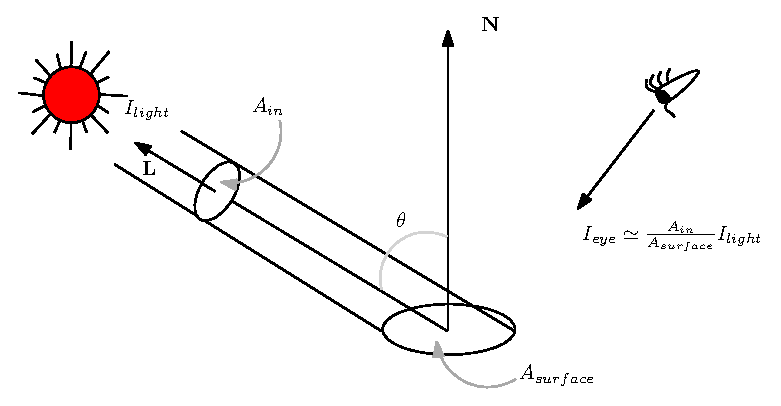
\includegraphics[height=6cm]{OGL_light/diffuseConcept.eps}
    \caption{난반사 광강도 결정 방법의 개념적 이해}
    \label{fig:OGL_light:diffuseConcept}
\end{figure}

이 값은 광원 벡터 $\mathbf L$과 법선 벡터 $\mathbf N$이 일치할 때 최대이며, 90도를 이룰 때 0이 된다. 이 값은 두 벡터의 내적, 
즉 두 벡터 사잇각의 코사인(cosine)에 비례한다는 것이 램버트 반사(Lambertian reflectance) 모델이다. \index{램버트 반사}\index{Lambertian reflection}
따라서 다음 식 \ref{eq:diffuseIntensity}과 같이 광강도를 계산해야하는 지점에서 빛을 향하는 방향벡터 $\mathbf L$과 
표면 법선벡터 $\mathbf N$의 내적으로  $I_d$를 구할 수 있다

\begin{eqnarray}
\label{eq:diffuseIntensity}
I_d  =  \cos \theta   = \mathbf L \cdot \mathbf N
\end{eqnarray}


\begin{figure}[h!]
  \centering
    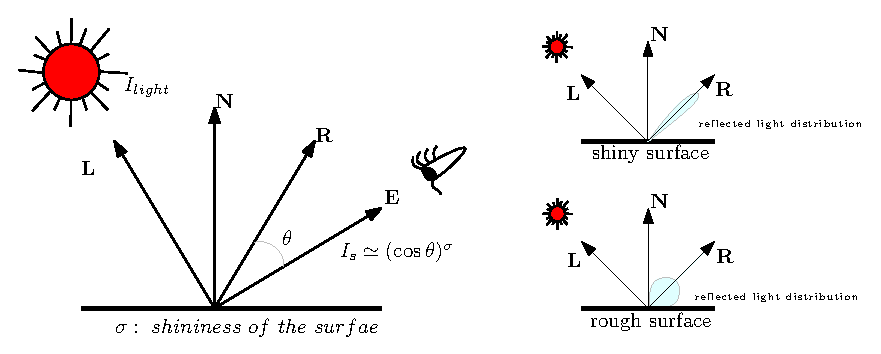
\includegraphics[height=5cm]{OGL_light/specularConcept.eps}
    \caption{정반사 광강도 결정 방법의 개념적 이해}
    \label{fig:OGL_light:specularConcept}
\end{figure}

정반사는 거울과 같이 입사각에 대칭되는 방향으로 반사되는 것이다. 그런데, 실제 물체들은 이런 이상적인 정반사가 아니라 반사 방향으로 빛이 강하게 진행하기는 하지만 다른 방향으로 조금씩 빛이 나간다. 퐁 모델에서 사용하는 정반사 모델은 거울과 같은 반사가 아니라 반사 벡터 $\mathbf R$ 중심으로 퍼지는 반사를 표현한다.

이 반사는 반사 벡터 $\mathbf R$ 근처에서 강하게 관찰되기 때문에 눈을  $\mathbf R$ 근처로 가져가야 강한 빛을 볼 수 있다. 
따라서 정반사의 광강도 $I_s$는 $\mathbf R$과 
$\mathbf E$의 사잇각의 코사인에 연관된다. 그리고 물체의 재질에 따라 $\mathbf R$ 방향으로 집중되는 정도가 달라진다. 
이것은 물체의 반질함(shininess)에 의해 결정되는데, 이 반질함을 $\sigma$라고 하자. 
그러면 이 반질함을 지수로 하는 모델을 만들 수 있다. 
그림 \ref{fig:OGL_light:specularConcept}는 이러한 정반사의 강도가 결정되는 방식을 개념적으로 보이고 있다.
이러한 개념을 수식으로 표현하면 식 \ref{eq:specularIntensity}와 같다.

\begin{eqnarray}
\label{eq:specularIntensity}
I_d  = \cos \theta =  (\mathbf R \cdot \mathbf E )^\sigma
\end{eqnarray}

주변광의 광강도는 언제나 1이다. 따라서 모든 물체는 다음과 같이 주변광과 주변광 반사 재질에 의한 색상
$\mathbf l_a \otimes \mathbf m_a$을 기본적으로 갖게 된다.  이것은 지역조명 기법의 단점인 지나치게 어두운 부분을 없애는 역할을 수행한다.
이상의 광강도를 모두 계산하고 나면 다음과 같이 최종적으로 어떤 지점이 눈에 어떠한 색상으로 보이는지를 결정할 수 있다. 해당 지점의 반사 색상, 
광원의 색상이 각 반사 요소별로 결정되어 있다고 할 때, 해당 지점은 식 \ref{eq:PhongModel2} 같은 색을 갖는다.

\subsection{수정된 퐁 모델 - 블린(Blinn) 모델}
\index{수정된 퐁 모델}\index{블린 모델}\index{퐁 모델!블린의 수정}
\index{modified Phong model}\index{Blinn model}\index{Phong model!modified}

\index{반벡터}\index{halfway vector}
퐁 모델은 정반사 광강도 계산에서 반사 벡터 $\mathbf R$을 계산해야 한다.
블린(Blinn)은 따로 이 반사벡터 대신에 반 벡터(halfway vector)라는 것을 도입하였다.
반 벡터 $\mathbf H$는 광원 벡터와 시선 벡터 $\mathbf E$를 더해서 다음과 같이 정규화하면 된다\cite{edward1997interactive}.
$$\mathbf H = \frac{\mathbf L + \mathbf E}{|\mathbf L + \mathbf E|}$$

이러한 반벡터의 개념과, 이를 활용하여 반사 벡터 없이 정반사 광강도를 계산할 수 있는 이유가 그림 \ref{fig:OGL_light:halfwayVector}에 나타나 있다.
\begin{figure}[h!]
  \centering
    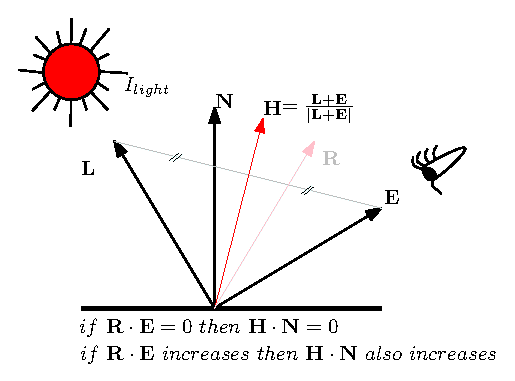
\includegraphics[height=6cm]{OGL_light/halfwayVector.eps}
    \caption{반벡터(halfway vector)의 개념}
    \label{fig:OGL_light:halfwayVector}
\end{figure}

정반사 광강도는 반사벡터 $\mathbf R$이 아니라, 
이 반 벡터를 이용하여 다음 식 \ref{eq:modifiedPhongModel}과 같이 구할 수 있다는 것이 블린(Blinn)이 제안한 수정 모델이다.


\begin{eqnarray}
\label{eq:modifiedPhongModel}
\kappa  =  \mathbf l_a \otimes \mathbf m_a + (\mathbf L \cdot \mathbf N) \mathbf l_d \otimes \mathbf m_d + 
(\mathbf H \cdot \mathbf N )^\sigma \mathbf l_s \otimes \mathbf m_s
\end{eqnarray}

\section{오픈지엘 조명 다루기}
\index{조명!오픈지엘}\index{light!OpenGL}

이 절에서는 실제 OpenGL 코드를 사용하여 물체에 조명을 비추는 작업을 수행할 것이다. 앞에서 다룬 퐁 모델은 우리가 특별한 코딩(coding)을 하지 않아도 OpenGL이 처리하여 준다. 우리가 설정해야 할 것은 조명을 사용할 것이라는 것과, 조명의 색과 물체의 색을 결정하는 것이다.
조명과 재질 설정
조명과 재질은 난반사(diffuse), 정반사(specular), 주변광(ambient)으로 구분하여 각각 설정해야 한다. 따라서 총 6 가지의 색상 설정이 필요하다. 그리고 재질의 반질거림(shininess)까지 설정하면 된다. 
다음으로 설정해야 하는 것은 조명의 위치이다. 조명의 위치는 동차좌표(homogeneous coordinate)로 표현하는데, 마지막 성분이 1이면 점광원이고, 0이면 방향광원(directional light source)라고 생각하면 된다.
다음과 같은 코드 \ref{code:OGL_light:preparingLightingData}를 살펴보자.

\begin{algorithmbis}[조명과 물체 재질로 입력할 값과 광원의 위치 결정]\label{code:OGL_light:preparingLightingData}
\lstset{language=C++, escapechar=^} 
\begin{lstlisting}
//^{\it 재질의 정반사, 난반사, 주변광, 반질거림 특성으로 사용될 데이터}^
// values for material specification
GLfloat mat_specular[] = { 1.0, 1.0f, 1.0f, 1.0f };
GLfloat mat_diffuse[] =  { 0.0, 1.0f, 1.0f, 1.0f };
GLfloat mat_ambient[] = { 1.0, 1.0, 1.0, 1.0 };
GLfloat mat_shininess[] = { 120.0 };
// ^{\it 광원의 정반사, 난반사, 주변광 특성으로 사용될 데이터}^
// values for light specification
GLfloat lit_specular[] = { 1.0,1.0f,1.0f,1.0f };
GLfloat lit_diffuse[] =  { 0.0,1.0f,1.0f,1.0f };
GLfloat lit_ambient[] =  { 0.5,0.0f,0.0f,1.0f };
// ^{\it 광원의 위치로 사용될 데이터}^
// values for light positioning
GLfloat light_position[] = {1.0,1.0f,1.0f,0.0f};
\end{lstlisting}
\end{algorithmbis}

이상의 코드는 실제로 광원과 재질을 설정하는 것이 아니라 값만 준비해 둔 것이다. 이 값들을 실재 조명과 재질에 적용해야 한다. 조명의 특성을 설정하는 
함수는 {\sf glLight*}이며, 재질 특성을 설정하는 것은 {\sf glMaterial*}이다. 
이를 이용하여 다음 코드 \ref{code:OGL_light:lightAndMaterial}과 같이 물체의 재질과, 광원의 특성을 설정한다.

이 코드를 살펴보면, 우선 {\sf LightSet} 함수는 조명과 재질의 색상을 지정한다. 그리고 나서 {\sf GL\_LIGHTING}을 활성화하여 오픈지엘(OpenGL)이 조명을 사용하도록 한다. 또한 오픈지엘 고정 파이프라인이 사용할 수 있는 조명 가운데 어떤 조명을 사용할 것인지를 설정하고 있다. 이 경우  {\sf GL\_LIGHT0} 하나만을 사용한다.
{\sf glLightPositioning}은 광원의 위치를 설정하고 있다. 이렇게 광원이 설정되면 법선 벡터를 가진 각 정점은 퐁 모델에 의해 그 밝기와 색상이 결정된다. 이때 법선 벡터를 지정하는 방법은 조금 뒤에 다루도록 하고, 법선 벡터가 포함된 그리기를 사용할 것이다. 이 경우에는 {\sf glutSolidTeapot}을 사용한다. 


\begin{algorithmbis}[조명과 재질 파라미터 입력 및 광원 위치 설정]\label{code:OGL_light:lightAndMaterial}
\lstset{language=C++, escapechar=^} 
\begin{lstlisting}
// ^{\it 조명과 재질의 특성을 준비된 데이터로 설정하는 함수}^
void LightSet(void) {
  glMaterialfv(GL_FRONT, GL_SPECULAR, mat_specular);
  glMaterialfv(GL_FRONT, GL_DIFFUSE, mat_diffuse);
  glMaterialfv(GL_FRONT, GL_AMBIENT, mat_ambient);
  glMaterialfv(GL_FRONT, GL_SHININESS, mat_shininess);

  glLightfv(GL_LIGHT0, GL_SPECULAR, lit_specular);
  glLightfv(GL_LIGHT0, GL_DIFFUSE, lit_diffuse);
  glLightfv(GL_LIGHT0, GL_AMBIENT, lit_ambient);
  glEnable(GL_LIGHTING);
  glEnable(GL_LIGHT0);
}

//^{\it 조명의 위치를 설정하는 함수}^
void LightPositioning(void) {
  glLightfv(GL_LIGHT0, GL_POSITION,light_position);
}
\end{lstlisting}
\end{algorithmbis}

이상과 같이 광원과 재질의 특성을 설정하는 함수를 작성한 뒤에
코드 \ref{code:OGL_light:FirstLighting}에 나타난 바와 같이 호출하면
그림 \ref{fig:OGL_light:firstLighting} (a)와 같은 결과를 얻을 수 있다.

\begin{algorithmbis}[조명과 재질 파라미터 입력 및 광원 위치 설정]\label{code:OGL_light:FirstLighting}
\lstset{language=C++, escapechar=^} 
\begin{lstlisting}
void init(int argc, char **argv) {
  ^{\sf [[각종 초기화 작업]]^
  LightSet(); // ^{\it 조명의 특성과 재질의 특성을 설정한다}^
  glEnable(GL_DEPTH_TEST);
}
void display() {
  ^{\sf [[GL\_MODELVIEW 모드 설정]]}^	
  gluLookAt(0,1,2,0,0,0,0,1,0);
  LightPositioning();  // ^{\it 점광원의 위치를 설정한다}^
  glutSolidTeapot(0.5);
  glutSwapBuffers();
}
\end{lstlisting}
\end{algorithmbis}


\begin{figure}[h!]
  \centering
    \begin{tabular}{cc}
	\fbox{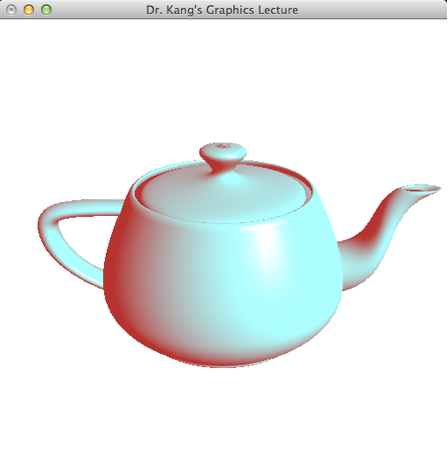
\includegraphics[height=4cm]{OGL_light/firstLighting.png}} &
	\fbox{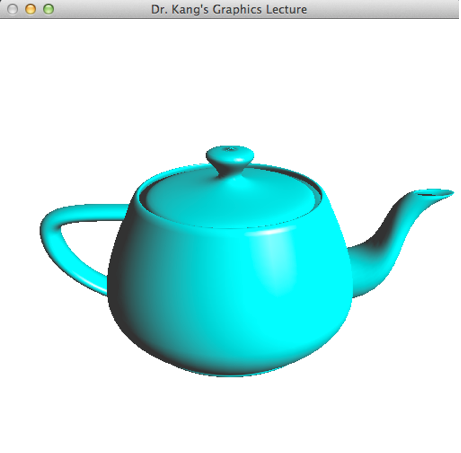
\includegraphics[height=4cm]{OGL_light/noAmbient.png}}\\
	\sf \small (a) 주변광 포함 & \sf \small (b) 주변광 제외 
	\end{tabular}
    \caption{오픈지엘 조명을 이용하여 그려낸 주전자}
    \label{fig:OGL_light:firstLighting}
\end{figure}

주변광을 제거하는 경우를 생각해 보자. 예를 들어, 광원의 주변광 색상을 (0,0,0,1)으로 바꾸면 주변광 요소는 없어진다. 이 경우 
그림 \ref{fig:OGL_light:firstLighting}의 주전자의 모습은 그림 \ref{fig:OGL_light:firstLighting} (b)와 같이 바뀐다.
그림에서 확인할 수 있는 바와 같이 주변광이 없으면 기본적으로 주어지는 밝기가 없기 때문에 조명에 의해 밝게 빛나는 부분과
그렇지 않은 부분의 명암 대비가 커지게 된다.


이번에는 반질거림의 정도를 변경해 볼 것이다. 물체는 당구공처럼 반질거리는 것도 있고,
고무공처럼 반질거림이 덜한 것도 있다. 반질거리는 정도의 차이는 하일라이트(highlight)에 의해
인지된다. 그런데 앞서 살펴본 난반사에서는 모든 방향으로 동일한 반사를 하기 때문에
이런 하일라이트를 표현할 수 없다. 정반사 모델에 대해서는 이미 살펴 보았으므로
실제 OpenGL 코드에서 이를 제어하는 방법을 살펴보자. 
아래 코드 \ref{code:OGL_light:specularControl}와 같이 {\sf display} 함수 내에서 
여러 주전자를 그리고, 오른쪽으로 갈수록 반질거림이 높아지도록 하였다. 결과는 그림 \ref{fig:OGL_light:specularControl}과 같다.

\begin{algorithmbis}[반질거림의 정도를 조절하기]\label{code:OGL_light:specularControl}
\lstset{language=C++, escapechar=^} 
\begin{lstlisting}
  for (int i=0; i<5; i++) {
       // ^{\it 재질의 반질거림을 변경하여 설정하고 주전자를 그림}^
       glMaterialf(GL_FRONT, GL_SHININESS, 4.0f+123.0f*(i/4.0)); 
       for (int j=0; j<5; j++) {
           glPushMatrix();
           glTranslated(float(i)+0.5, float(j)+0.5, 0.0);
           glRotated(45, 1, 1, 1);
           glutSolidTeapot(0.4);
           glPopMatrix();
      }
  }
\end{lstlisting}
\end{algorithmbis}

\begin{figure}[h!]
  \centering
    \fbox{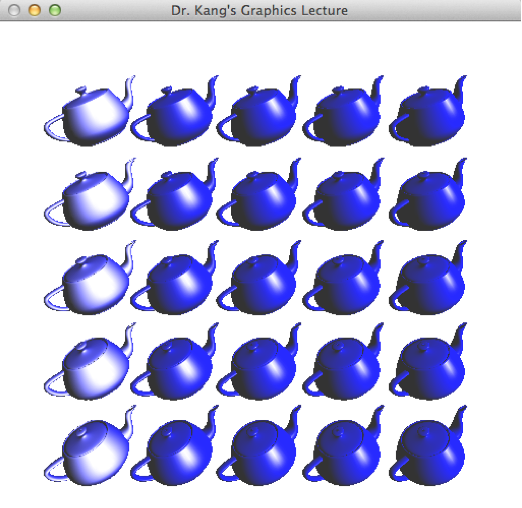
\includegraphics[height=6cm]{OGL_light/specularControl.png}}
    \caption{오픈지엘 조명을 이용하여 그려낸 주전자에서 정반사를 제어한 결과}
    \label{fig:OGL_light:specularControl}
\end{figure}

\subsection{점광원의 구현}

지금까지 살펴본 광원은 ``방향광원(directional light)"였다.
이것은 코드 \ref{code:OGL_light:preparingLightingData}에 나타나 있는 광원의 위치를 통해 확인할 수 있다.
여기에는 광원의 위치가 동차좌표계로 표현되어 있고, 그 $w$ 좌표가 0으로 설정되어 있다.
이것은 앞서 동차좌표계에서 다루었던 것처럼 3차원 공간의 어떤 점이 아니라 벡터를 의미하는 것이다.
따라서 그림 \ref{fig:OGL_light:specularControl}에서 확인할 수 있는 것처럼 모든 객체가 동일한 방향에서 오는 빛을 받아
음영이 그려지게 된다.

방향광원은 햇볕과 같은 빛을 표현하는 데에 적합하다. 그런데 많은 경우 전구와 같이 하나의 점에서 빛이 모든 방향으로 퍼져 나가는
경우도 표현할 필요가 있다. 이렇게 한 점에서 모든 방향으로 빛이 퍼지는 광원을 점광원(point light)라고 한다.
점광원을 구현하는 방법은 광원의 좌표에서 $w$ 성분을 0이 아닌 값, 일반적으로는 1을 설정하면 된다.
코드 \ref{code:OGL_light:pointLight}는 이러한 OpenGL로 구현한 예이다.

이 코드를 실행할 경우 그림 \ref{fig:OGL_light:pointLight}와 같은 결과를 얻을 수 있다. 그림에서 확인할 수 있는 바와 같이
광원의 위치가 3차원 공간에 있고, 각각의 객체는 이 광원으로부터 서로 다른 방향의 빛을 받게 된다.

\begin{figure}[h!]
  \centering
    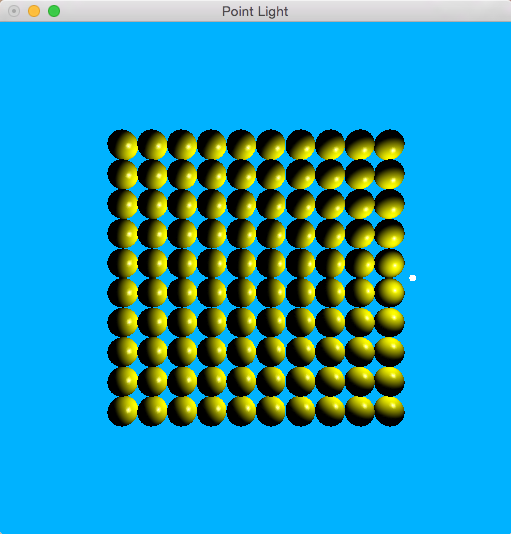
\includegraphics[height=8cm]{OGL_light/pointLight.png}
    \caption{점광원을 설정한 결과}
    \label{fig:OGL_light:pointLight}
\end{figure}

\begin{algorithmbis}[점광원 구현하기]\label{code:OGL_light:pointLight}
\lstset{language=C++, escapechar=^} 
\begin{lstlisting}
^{\sf [[광원과 재질의 색상 설정]]}^
// ^{\it 광원의 위치를 설정한다.}^
// ^{\it 광원의 좌표 가운데 w 성분이 1로 설정되어 있다}^
// ^{\it 디스플레이 콜백에서 광원의 위치를 바꾸지만, w 좌표는 변경하지 않는다}^
GLfloat lit_position[] = { 0.0f, 0.0f, 0.0f, ^{\bf 1.0f}^ }; // light position

void SetLight() {    ^{\sf 이전 코드와 동일}^  }

void init(void) {
    ^{\sf [[윈도우, 버퍼 초기화, 카메라 설정 등의 초기 작업]]}^
    SetLight();
}

void display() {
    // ^{\sf [[버퍼 지우기, 모델뷰 행렬 모드 설정, 카메라 위치 설정 등 수행]]}^
    static float t = 0.0; t+=0.01;
    // ^{\it 광원의 위치를 설정함. w 좌표는 1로 고정하고 회전하도록 함}^
    lit_position[0] = 5.0*sin(t); lit_position[2] = 5.0*cos(t);
    glLightfv(GL_LIGHT0, GL_POSITION, lit_position);

    for(int i=0;i<10;i++) {
        for(int j=0;j<10;j++) {
            glPushMatrix();
            glTranslatef(i-4.5,j-4.5,0);
            glutSolidSphere(0.5, 30, 30);
            glPopMatrix();
        }
    }
    // ^{\sf [[광원의 위치 등을 표시하여 확인할 수 있도록 함]]}^
    glutSwapBuffers();
}
\end{lstlisting}
\end{algorithmbis}

\subsection{집중광원의 구현}

집중광원은 탐조등(探照燈)처럼 특정한 방향으로 빛을 집중하여 보내는 것이다.
이러한 집중광원은 점광원의 특징에 몇 가지 제약을 주면 된다.
그림 \ref{fig:OGL_light:spotLight}에 보인 것처럼, 집중광원은 광원이 진행하는 방향을 나타내는
{\sf GL\_SPOT\_DIRECTION}과, 빛이 퍼지는 범위의 한계를 설정하는 {\sf GL\_SPOT\_CUTOFF}가 필요하다.

\begin{figure}[h!]
  \centering
    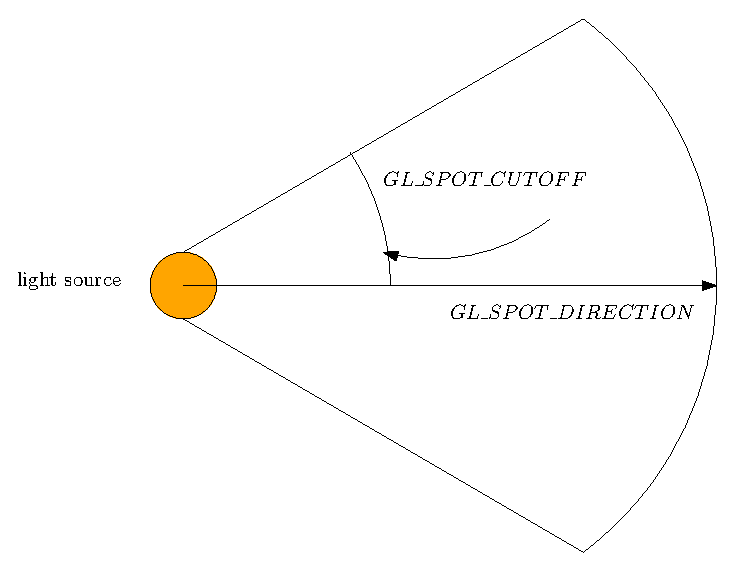
\includegraphics[height=7cm]{OGL_light/spotLight.eps}
    \caption{집중광원에 필요한 추가 요소들}
    \label{fig:OGL_light:spotLight}
\end{figure}

이러한 설정을 추가하여 코드 \ref{code:OGL_light:pointLight}를 개선한 다음과 같은 
코드 \ref{code:OGL_light:spotLight}를 구현할 수 있다.

\begin{algorithmbis}[집중 광원 구현하기]\label{code:OGL_light:spotLight}
\lstset{language=C++, escapechar=^} 
\begin{lstlisting}
// ^{\it 집중 광원의 방향으로 사용될 데이터를 준비한다}^
GLfloat spotDir[] = { 0.0f, 0.0f, -1.0f };

void SetLight() {
    glEnable(GL_LIGHTING);
    glEnable(GL_LIGHT0);
    // set material properties
    glMaterialfv(GL_FRONT, GL_DIFFUSE, mat_diffuse);
    glMaterialfv(GL_FRONT, GL_SPECULAR, mat_specular);
    glMaterialfv(GL_FRONT, GL_AMBIENT, mat_ambient);
    glMaterialfv(GL_FRONT, GL_SHININESS, mat_shininess);

    // set light properties
    glLightfv(GL_LIGHT0, GL_DIFFUSE, lit_diffuse);
    glLightfv(GL_LIGHT0, GL_SPECULAR, lit_specular);
    glLightfv(GL_LIGHT0, GL_AMBIENT, lit_ambient);

    // ^{\it 집중광원에 필요한 데이터를 설정한다}^    
    glLightf (GL_LIGHT0,GL_SPOT_CUTOFF,20.0f);
    glLightfv(GL_LIGHT0,GL_SPOT_DIRECTION,spotDir);
    // ^{\it Exponent 집중광의 테두리를 부드럽게 한다. 자세한 내용은 Reference API 등을 참고하라}^
    glLightf (GL_LIGHT0,GL_SPOT_EXPONENT, 20.0f);

}
\end{lstlisting}
\end{algorithmbis}

코드 \ref{code:OGL_light:spotLight}를 실행한 결과는 그림 \ref{fig:OGL_light:spotLightResult}에 나타나 있다.

\begin{figure}[h!]
  \centering
    \fbox{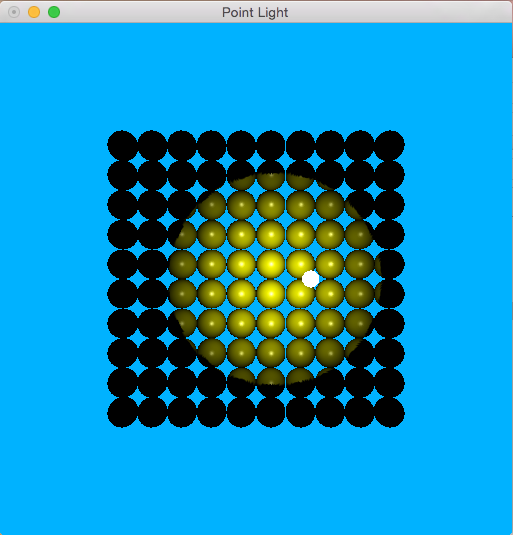
\includegraphics[height=8cm]{OGL_light/spotLight.png}}
    \caption{집중광원 구현 결과}
    \label{fig:OGL_light:spotLightResult}
\end{figure}

\section{법선의 설정과 메시(mesh) 데이터 그리기}

앞서 그려본 주전자는 그려지는 면의 법선 벡터가 내장되어 있는 {\sf glutSolidTeapot} 함수를 호출하여 그렸다. 그런데 임의의 면을 그릴 때는 이러한 미리 정의된 법선 벡터가 존재하지 않는다. 그렇다면 퐁 쉐이딩의 계산이 요구되는 법선 벡터는 어떻게 오픈지엘에 넘겨줄 수 있을까?
우선 법선 벡터를 어디에 지정해야 하는지를 생각해 보자. 각각의 정점은 자신의 색을 가져야 하며, 이 색은 퐁 모델을 통해 계산된다. 이때 법선 벡터가 필요하므로 각 정점마다 법선 벡터를 지정해야 한다. 그러면, 각 정점이 아니라 이 정점들이 만드는 다각형의 내부 각 점들은 어떠한가? 각 점들 역시 물체 위의 표면을 나타내며, 각각 색을 결정해야 하므로 법선벡터가 필요하다. 그런데, 일일이 이런 모든 점을 표현하는 픽셀 하나 하나에 법선을 설정하는 것은 거의 불가능하다. 따라서 오픈지엘은 그림
\ref{fig:OGL_light:interpolatedColors}와 같이 다각형을 구성하는 꼭지점에서의 색을 구한 뒤에 다각형 내부의 색은 이 색들을 보간하여 결정한다.

그림의 한 면은 세 개의 정점으로 이루어져 있다. 각 정점은 법선 벡터를 가지고 있고, 이 법선 벡터와 조명의 관계를 이용하여 퐁 쉐이딩을 할 수 있다. 그러면 우리는 각 정점의 색을 얻을 수 있다. 그리고 이렇게 얻어진 정점의 색을 이용하여 내부의 특정 픽셀은 선형보간(linear interpolation)을 통해 얻으면 쉽게 내부의 색을 칠할 수 있다. 이러한 내부 색칠 방식을 구로(Gouraud) 쉐이딩이라고 한다. \index{구로 세이딩}\index{Gouraud shading}

\begin{figure}[h!]
  \centering
    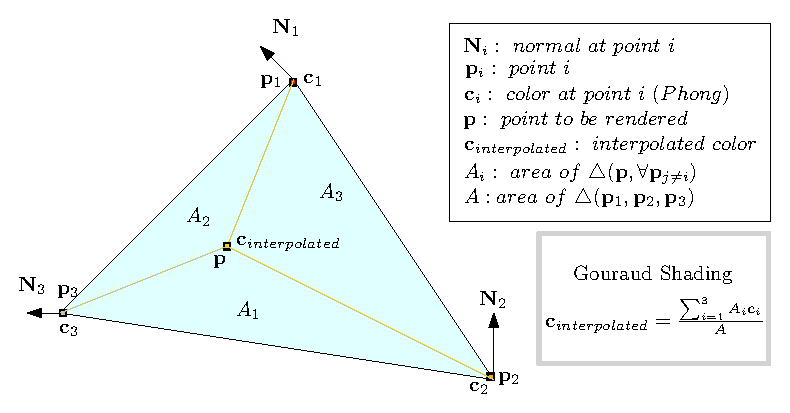
\includegraphics[height=7cm]{OGL_light/interpolatedColors.eps}
    \caption{구로(Gouraud) 세이딩의 계산 방법}
    \label{fig:OGL_light:interpolatedColors}
\end{figure}

구로 세이딩을 할 대상이 그림 \ref{fig:OGL_light:interpolatedColors}와 같이 $\mathbf p_1$, $\mathbf p_2$, $\mathbf p_3$와 같이 세 개의 정점으로 이루어진
삼각형이라고 하자. 각각의 정점에서 가지는 법선 벡터는 $\mathbf N_1$, $\mathbf N_2$, $\mathbf N_3$로 표시하자.
앞에서 살펴본 퐁 모델을 이용하여 각 정점의 색 $\mathbf c_1$, $\mathbf c_2$, $\mathbf c_3$를 계산할 수 있다.
이렇게 계산된 색을 보간하는 것이 구로 세이딩이다. 이때 우리가 색을 칠하려고 하는 대상이 $\mathbf p$라고 하자.
이 지점은 보간된 색상 $\mathbf c_{interpolated}$를 가질 것이다.
이를 계산하기 위해서는 각각의 정점 색깔을 어떤 가중치(weight)로 혼합할 것인지를 결정해야 한다.
삼각형 $\triangle (\mathbf p_1, \mathbf p_2, \mathbf p_3 )$는 정점 $\mathbf p$를 각 정점으로 연결한 선분을 이용하여
그림 \ref{fig:OGL_light:interpolatedColors}처럼 세 구역으로 나뉜다. 하나의 구역은 세 정점 가운데 한 정점 $i$를 뺀 나머지 
두 정점과 그리려는 지점 $\mathbf p$를 연결하여 얻을 수 있고, 이 영역의 넓이를 빠진 정점 $i$의 번호를 달아 $A_i$로 표현하자.
그 이유는 이 영역의 크기가 커지면 $\mathbf p$가 $i$ 지점에 가까워지고, 색도 $\mathbf c_i$에 가까워져야 하기 때문이다.
즉, 이 크기는 색상 $\mathbf c_i$에 곱해지는 가중치로 쓸 수 있다.

구로 세이딩은 보간된 색상 $\mathbf c_{interpoalted}$를 다음과 같이 구한다.

\begin{eqnarray}
\mathbf c_{interpolated} = \frac{\sum_{i=1}^3 A_i \mathbf c_i}{A}
\end{eqnarray}




\begin{figure}[h!]
  \centering
    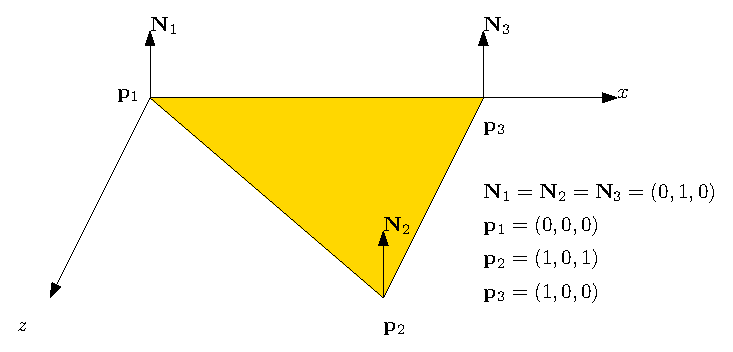
\includegraphics[height=6cm]{OGL_light/simpleTriangle.eps}
    \caption{구로(Gouraud) 세이딩의 계산 방법}
    \label{fig:OGL_light:simpleTriangle}
\end{figure}

이제 간단한 면을 오픈지엘로 렌더링(rendering)해 보자.
간단한 삼각형 하나를 그릴 것이다. 삼각형은 세 개의 정점으로 구성되며, 각 정점은 자기 자신의 정점 좌표를 가진다. 
이 정점 좌표는 이미 {\sf glVertex*} 함수를 통해 지정하는 방법을 사용해 왔다. 이제 각 정점의 법선을 지정하는 방법이 필요하다. 
정점의 법선은 {\sf glNormal*} 함수를 이용하여 설정할 수 있다. 예를 들면 다음 그림 \ref{fig:OGL_light:simpleTriangle}에 나타난 
삼각형을 그린다고 할 때는 아래와 같이 입력한다.

\begin{verbatim}
glNormal3f(0,1,0); glVertex3f(0,0,0);
glNormal3f(0,1,0); glVertex3f(1,1,0);
glNormal3f(0,1,0); glVertex3f(1,0,0);
\end{verbatim}

이제 간단한 면을 그리는 코드 \ref{code:OGL_light:opengl_normalvectors}를  같이 작성해 보자. 이 코드의 실행 결과는 그림 \ref{fig:OGL_light:normalSetting}와 같다. 

\begin{algorithmbis}[삼각형 정점에 법선 부여하기]\label{code:OGL_light:opengl_normalvectors}
\lstset{language=C++} 
\begin{lstlisting}
  glBegin(GL_TRIANGLES);
  glNormal3f(0,1,0);
  glVertex3f(0,0,0);
  glNormal3f(2/sqrt(3),1/sqrt(3),0);
  glVertex3f(2,0,0);
  glNormal3f(-2/sqrt(3),1/sqrt(3),0);
  glVertex3f(1,0,-1);
  glEnd();
\end{lstlisting}
\end{algorithmbis}

\begin{figure}[h!]
  \centering
    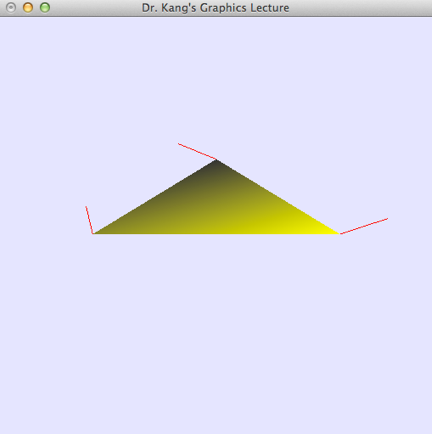
\includegraphics[height=5.5cm]{OGL_light/normalSetting.png}
    \caption{정점별로 법선 벡터를 설정하여 삼각형 그리기 수행 결과}
    \label{fig:OGL_light:normalSetting}
\end{figure}

그림 \ref{fig:OGL_light:normalSetting}의 결과는 코드 \ref{code:OGL_light:opengl_normalvectors}에는 없지만,
설정된 법선벡터를 가시화하기 위한 코드를 추가하여 실행한 결과이며, 각 정점에 설정된 법선 벡터가 선분으로 그려져 있다.
법선벡터가 다르기 때문에 퐁 모델에 의해 각 정점이 서로 다른 색으로 칠해지며,
삼각형 내부는 구로 세이딩을 통해 보간된 색으로 칠해진다.

이제 두 개의 인접한 면을 그려보자. 우선은 각각의 면에 하나씩 법선을 설정하는
코드 \ref{code:OGL_light:twoFacesTwoNormals}와 같이 그려보자. 결과는 그림 \ref{fig:OGL_light:twoFacesTwoNormals}와 같다.

\begin{algorithmbis}[두 개의 면 그리기]\label{code:OGL_light:twoFacesTwoNormals}
\lstset{language=C++} 
\begin{lstlisting}
  glBegin(GL_TRIANGLES);
  glNormal3f(-1/sqrt(2),1/sqrt(2),0);
  glVertex3f(0,1,0);
  glVertex3f(-1,0,0);
  glVertex3f(0,1,1);
  glNormal3f(1/sqrt(2),1/sqrt(2),0);
  glVertex3f(0,1,0);
  glVertex3f(0,1,1);
  glVertex3f(1,0,0);
  glEnd();
\end{lstlisting}
\end{algorithmbis}

\begin{figure}[h!]
  \centering
    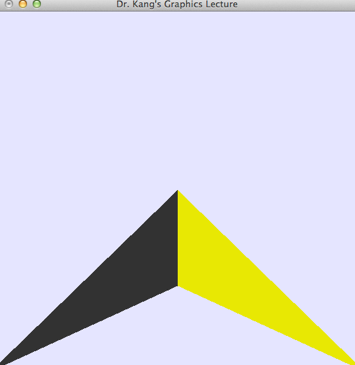
\includegraphics[height=6.0cm]{OGL_light/twoFacesTwoNormals.png}
    \caption{두 개의 면을 서로 다른 두 법선 벡터로 그린 결과}
    \label{fig:OGL_light:twoFacesTwoNormals}
\end{figure}

이렇게 면 별로 서로 다른 법선을 주면 경계가 부드럽게 표현되지 않는다. 이때 두 면에 공유되는 가운데 
두 점은 양쪽 면을 모두 고려하여 (0,1,0)으로 설정하면 다음과 같은 코드 \ref{code:OGL_light:twoFacesFourNormals}처럼 작성할 수 있다.
 실행 결과는 그림 \ref{fig:OGL_light:twoFacesFourNormals}에 보이고 있다.

\begin{algorithmbis}[공유된 점에 공통 법선 부여]\label{code:OGL_light:twoFacesFourNormals}
\lstset{language=C++} 
\begin{lstlisting}
  glBegin(GL_TRIANGLES);
  glNormal3f(0,1,0);  
  glVertex3f(0,1,0);
  glNormal3f(-1/sqrt(2),1/sqrt(2),0);  
  glVertex3f(-1,0,0);
  glNormal3f(0,1,0);  
  glVertex3f(0,1,1);
  glNormal3f(0,1,0);  
  glVertex3f(0,1,0);
  glNormal3f(0,1,0);  
  glVertex3f(0,1,1);
  glNormal3f(1/sqrt(2),1/sqrt(2),0);  
  glVertex3f(1,0,0);
  glEnd();
\end{lstlisting}
\end{algorithmbis}

\begin{figure}[h!]
  \centering
    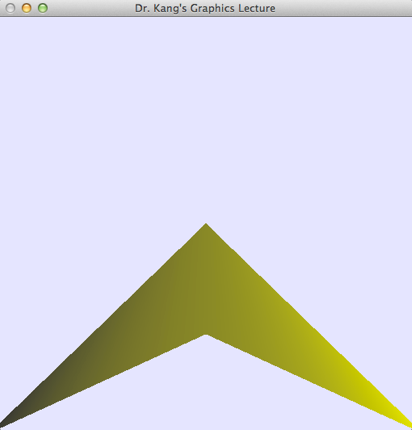
\includegraphics[height=5cm]{OGL_light/twoFacesFourNormals.png}
    \caption{각각의 정점에 서로 다른 법선을 적용}
    \label{fig:OGL_light:twoFacesFourNormals}
\end{figure}

\subsection{메시 읽고 그리기}\index{mesh}\index{메시}

이제 우리는 임의의 메시를 읽고 법선을 계산하여 조명을 비추는 작업을 수행할 것이다.
우선 간단한 메시 데이터 포맷을 정의하자. 
우리의 메시 데이터는 표 \ref{tab:meshDataExample}와 같은 형태를 가진다. 
파일의 가장 처음에 나타나는 것은 전체 정점의 개수 $n$이다. 
그리고 모두 $n$ 개의 정점에 대해 위치 정보가 3차원 벡터로 나타난다.
그 다음은 면의 개수 $m$이 온다. 그리고 이어지는 정보는
$m$ 개의 면이 가진 정점 정보를 보여준다.
하나의 면은 삼각형으로 이루어지고, 면을 표현하는 정보는 이 삼각형을 구성하는
정점의 번호 세 개가 나타난다.
하나의 정점은 1에서 $n$ 사이의 정수 하나로 표현할 수 있다. 
오른쪽 칼럼의 내용은 우리가 앞서 그려본 도형을 메시 파일로 표현한 것이다.


\begin{table}
\caption{메시 데이터 포맷의 예시}
\label{tab:meshDataExample}
\begin{center}
    \begin{tabular}{ |l|l|}
    \hline
    {\small \sf 포맷} & {\small \sf 실제 데이터 예시} \\ \hline
\pbox{10cm}{\small \sf numVertices $n$\\ vertex 1 ($x_1,y_1,z_1$)\\ vertex 2 ($x_2,y_2,z_2$)\\ ...\\ vertex $n$ ($x_n,y_n,z_n$)\\ numFaces $m$\\ face 1 ($f_1.v_1,f_1.v_2,f_1.v_3$)\\ face 2 ($f_2.v_1,f_2.v_2,f_2.v_3$)\\ ...\\ face m ($f_m.v_1,f_m.v_2,f_m.v_3$)} & 
\pbox{10cm}{\small \sf 4\\ 0.0 1.0  0.0\\ -1.0  0.0  0.0\\  0.0  1.0  1.0\\  1.0  0.0  0.0\\ 2\\ 0 1 2\\  0 2 3 } \\ 
\hline
\end{tabular}
\end{center}
\end{table}

이러한 메쉬를 읽어 들이는 클래스를 작성해 보자. 우선 헤더 파일에서 클래스의 기본적인 설계를 해 보자. 다음 코드 \ref{code:OGL_light:meshClass}와 같은 구조가 될 것이다.
이 메쉬 클래스는 {\sf cvertex}라는 정점 데이터를 저장하는 클래스와, 면 데이터를 저장하는 {\sf cface} 클래스를 먼저 정의한다. 정점은 3차원 좌표이다. 면은 세 개의 정점으로 구성되는데, 정점의 좌표나 정점 객체를 그대로 쓰는 것이 아니라 정점이 저장된 배열의 색인(index)로 표현한다. 
메쉬 클래스에서 가장 중요한 데이터는 정점 데이터이다. 메쉬 전체를 이루는 정점의 개수와 면의 개수가 멤버 변수로 있고, 정점은 {\sf cvertex} 형 배열로 다뤄진다. 면은 {\sf cface} 형 배열이다. 추가로 사용되는 데이터는 메쉬를 읽고 나서 전체적인 크기를 파악할 수 있는 바운딩 박스 정보이다. 축정렬(axis-aligned) 바운딩 박스를 사용하여 {\sf minx, miny, minz, maxx, maxy, maxz}의 값으로 표현된다. 외부 인터페이스로는 생성자와 함께, 메쉬를 읽는 {\sf loadMesh}, 메쉬를 그리는 {\sf drawMesh} 두 함수만 있다.


\begin{algorithmbis}[메시 클래스 정의]\label{code:OGL_light:meshClass}
\lstset{language=C++, escapechar=^} 
\begin{lstlisting}
#ifndef _mesh_sms_hh_
#define _mesh_sms_hh_
class cvertex {
public:
    float x;
    float y;
    float z;
}; // ^{\it 하나의 점을 구성하는 좌표값 3 개}^
class cface {
public:
    int v0; int v1; int v2;
}; //^{\it 하나의 삼각형 면을 구성하는 세 개 정점의 인덱스들}^

class CMesh {
    int nV;  // ^{\it 정점의 개수}^
    int nF;  // ^{\it 메시 구성 삼각형 면의 수}^
    cvertex *v; // ^{\it 정점 데이터 배열}^
    cface   *f; // ^{\it 면 데이터 배열}^

public:
    float minx, miny, minz;
    float maxx, maxy, maxz; // ^{\it 메시를 둘러싸는 AABB 경계상자}^

public:
    CMesh();  // constructor
    ~CMesh(); // destructor
    // ^{\it 메시를 읽고 그리는 메소드들}^
    void loadMesh(char *meshFileName);
    void drawMesh(void);
};
#endif
\end{lstlisting}
\end{algorithmbis}

이제 {\sf mesh.cpp} 파일을 작성할 것이다. 우선 생성자와 메쉬를 읽어들이는 코드를 작성해 보자. 생성자는 정점와 면의 개수를 0으로 설정하고, 정점과 면 데이터를 저장할 배열을 {\sf NULL}로 설정한다. 또한 바운딩 박스 데이터에서 {\sf min} 값을 매우 큰 음수로, {\sf max}는 매우 큰 값으로 설정해 둔다.

메쉬 파일을 읽어 들이는 {\sf loadMesh} 역시 매우 간단하다. 파일을 열고, 처음으로 정점의 개수를 {\sf nV}로 읽어 들인다. 
그리고 이 {\sf nV} 개수 만큼의 배열을 생성한 뒤에 차례로 좌표를 읽어 저장한다. 이때 좌표를 보고 {\sf min, max} 값들을 변경한다. 
다음으로 면의 개수를 읽어 들여 {\sf nF}에 저장하고, {\sf nF} 개의 면에 대해 각각 세 개 씩의 정점 색인을 읽어 저장한다.
코드 \ref{code:OGL_light:meshImplementation}와 같이 구현이 가능하다.

\begin{algorithmbis}[메시 클래스 구현]\label{code:OGL_light:meshImplementation}
\lstset{language=C++,escapechar=^} 
\begin{lstlisting}
#include "Mesh.h" 

^{\sf [[필요한 헤더 파일들 포함]]}^

#define BIGNUMBER 100000000000000000000000.0

CMesh::CMesh() : nV(0), nF(0), v(NULL), f(NULL),
    minx( BIGNUMBER), miny( BIGNUMBER), minz( BIGNUMBER),
    maxx(-BIGNUMBER), maxy(-BIGNUMBER), maxz(-BIGNUMBER) { }

CMesh::~CMesh() {
    if(v) delete[] v;
    if(f) delete[] f;    
}

void CMesh::loadMesh(char *meshFileName) {
    FILE *fptr = fopen(meshFileName, "r");
    if(!meshFileName || !fptr) {     
       printf("file open error\n"); exit(0);    
    }

    // ^{\it 정점의 개수 읽기}^
    fscanf(fptr, "%d", &nV);
    v = new cvertex[nV];
    for (int i=0; i<nV; i++) {
        // ^{\it {\sf nV}개의 정점 정보를 읽음}^
        fscanf(fptr, "%f", &v[i].x); 
        fscanf(fptr, "%f", &v[i].y); 
        fscanf(fptr, "%f", &v[i].z);
    }

    // ^{\it 면의 개수 읽기}^
    fscanf(fptr, "%d", &nF);
    f = new cface[nF];
    for (int i=0; i<nF; i++) {
        // ^{\it {\sf nF}개의 면 정보를 읽음}^
        fscanf(fptr, "%d", &f[i].v0);   
        fscanf(fptr, "%d", &f[i].v1);    
        fscanf(fptr, "%d", &f[i].v2);
    }
}
\end{lstlisting}
\end{algorithmbis}

그림을 그리는 {\sf drawMesh}는 다양한 방법으로 구현이 가능하다. 우선 읽어 들인 정점을 그대로 화면에 찍어 보는 다음과 같이
메시를 구성하는 정점을 출력하는 코드 \ref{code:OGL_light:meshVertexDraw}를 작성해 보자.


\begin{algorithmbis}[정점 화면 출력]\label{code:OGL_light:meshVertexDraw}
\lstset{language=C++} 
\begin{lstlisting}
void CMesh::drawMesh(void) {
  if(!v || !f) return;
  glBegin(GL_POINTS);
  for(int i=0;i<nV;i++) {
    glVertex3f( v[i].x, v[i].y, v[i].z);
  }
  glEnd();
}
\end{lstlisting}
\end{algorithmbis}

이 코드 \ref{code:OGL_light:meshVertexDraw}를 실행하면 
그림 \ref{fig:OGL_light:drawMeshVerts}와 같은 결과를 얻을 수 있다.

\begin{figure}[h!]
  \centering
    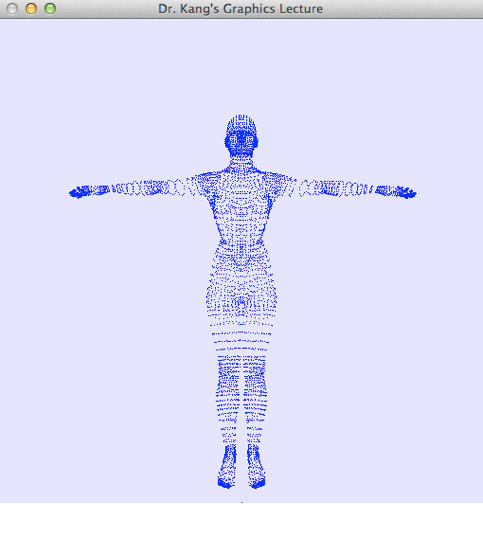
\includegraphics[height=6cm]{OGL_light/drawMeshVerts.png}
    \caption{메시의 정점을 그린 결과}
    \label{fig:OGL_light:drawMeshVerts}
\end{figure}

메쉬의 drawMesh 함수를 변경하여 각 면을 그리도록 코드를 코드 \ref{code:OGL_light:meshEdgeDraw}와 같이 변경해 보자.

\begin{algorithmbis}[메시의 간선을 그리기]\label{code:OGL_light:meshEdgeDraw}
\lstset{language=C++, escapechar=^} 
\begin{lstlisting}
void CMesh::drawMesh(void) {
    for (int i=0; i<nF; i++) {
        // ^{\it i-번째 면을 그리는 작업}^
        int a, b, c; // ^{\it 삼각형을 구성하는 세 정점의 인덱스}^
        a = f[i].v0; // ^{\it i-번째 면의 0번 정점}^
        b = f[i].v1; // ^{\it i-번째 면의 1번 정점}^
        c = f[i].v2; // ^{\it i-번째 면의 2번 정점}^
        glBegin(GL_LINE_LOOP);
        glVertex3f(v[a].x, v[a].y, v[a].z); // ^{\it a 정점의 좌표}^
        glVertex3f(v[b].x, v[b].y, v[b].z);// ^{\it b정점의 좌표}^
        glVertex3f(v[c].x, v[c].y, v[c].z); // ^{\it c 정점의 좌표}^
        glEnd();
    }
}
\end{lstlisting}
\end{algorithmbis}

이 코드는 점이 아니라 면을 그리며, 각 면이 가진 세 개의 색인을 이용하여 정점 배열에서 좌표를 얻어온다. 
결과는 그림 \ref{fig:OGL_light:meshEdgeDraw}와 같다.

\begin{figure}[h!]
  \centering
    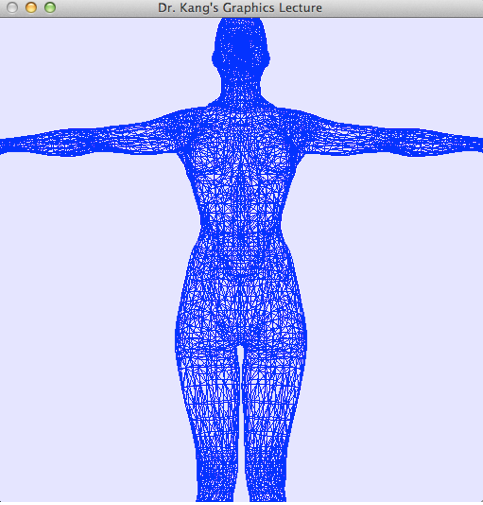
\includegraphics[height=10cm]{OGL_light/meshEdgeDraw.png}
    \caption{메시의 간선(edge)들을 그린 결과}
    \label{fig:OGL_light:meshEdgeDraw}
\end{figure}

다음으로 이 메쉬를 와이어프레임(wireframe) 구조가 아니라 채워진 면을 그리고자 한다. 면을 그릴 때에는 각 면이 조명을 받아 어떤 색상과 밝기를 갖는지가 결정되어야 한다. 조명 설정은 앞의 절에서 살펴본 방식대로 하면 될 것이다. 이 조명 환경에서 각각의 면들이 가진 밝기를 계산하기 위해서는 법선 벡터가 필요하다. 어떤 면의 법선 벡터를 구하는 것은 그 면 위의 서로 다른 두 벡터를 구해 외적한 뒤 정규화하면 된다.

하나의 삼각형에는 세 개의 정점이 있고, 한 정점에서 다른 어떤 정점의 좌표를 빼면 평면 위에 있는 벡터가 된다. 따라서 좌표가 주어진 삼각형 정점 세 개에서 두 개의 벡터를 구하는 것은 매우 간단한 일이다. 이 두 벡터를 외적하여 법선을 구할 수 있다. 

각각의 면을 그리면서 {\sf GL\_TRIANGLES} 프리미티브를 이용하여 채워진 면이 그려지도록 하며, 
이때 각 점의 법선은 앞서 설명한 방법으로 계산하여 그리도록 하는 코드는 다음의 코드 \ref{code:OGL_light:meshFlatSurfaces}와 같다.

\begin{algorithmbis}[법선을 계산하여 메시의 면을 그리기]\label{code:OGL_light:meshFlatSurfaces}
\lstset{language=C++, escapechar=^} 
\begin{lstlisting}
void CMesh::drawMesh(void) {

    if(!v || !f) return;
    glBegin (GL_TRIANGLES) ; 

    for(int i=0;i<nF;i++) {

        // ^{\it 법선 벡터를 계산하기 위한 정보}^
        cvertex p0, p1, p2;  // ^{\it 세 개의 정점 ${\mathbf p}_0, {\mathbf p}_1, {\mathbf p}_2$}^
        cvertex v0, v1; cvertex n; //^{\it 면 위의 두 벡터 ${\mathbf v}_0, {\mathbf v}_1$와 법선벡터 $\mathbf n$}^
        p0 = v[f[i].v0];
        p1 = v[f[i].v1];
        p2 = v[f[i].v2];

        // ^{\it ${\mathbf v}_0 = {\mathbf p}_1 - {\mathbf p}_0$}^
        v0.x = p1.x-p0.x; v0.y = p1.y-p0.y; v0.z = p1.z-p0.z; 
        // ^{\it ${\mathbf v}_1 = {\mathbf p}_2 - {\mathbf p}_0$}^
        v1.x = p2.x-p0.x; v1.y = p2.y-p0.y; v1.z = p2.z-p0.z;

        // ^{\it ${\mathbf n} = \frac{{\mathbf v}_1 \times {\mathbf v}_0}{|{\mathbf v}_1 \times {\mathbf v}_0|}$}^
        n.x = v0.y*v1.z-v0.z*v1.y;
        n.y = v0.z*v1.x-v0.x*v1.z;
        n.z = v0.x*v1.y-v0.y*v1.x;
        float len = sqrt(n.x*n.x+n.y*n.y+n.z*n.z); 
        n.x /= len; n.y /= len; n.z /= len;

        glNormal3f(n.x, n.y, n.z); 
        glVertex3f( p0.x, p0.y, p0.z); 
        glVertex3f( p1.x, p1.y, p1.z); 
        glVertex3f( p2.x, p2.y, p2.z);
    }
    glEnd() ;

}
\end{lstlisting}
\end{algorithmbis}

이 코드 \ref{code:OGL_light:meshFlatSurfaces}를 실행한 결과가
그림 \ref{fig:OGL_light:meshFlatSurfaces}에 나타나 있다.

\begin{figure}[h!]
  \centering
    \fbox{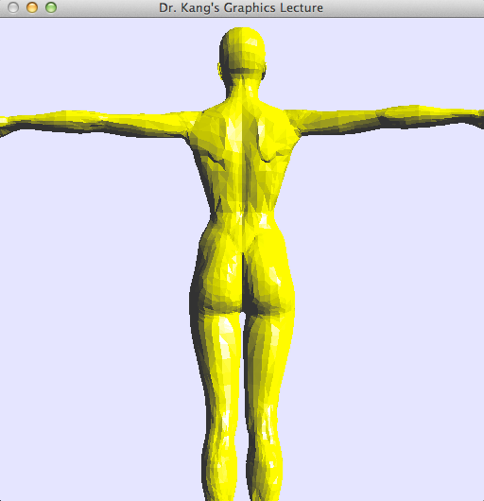
\includegraphics[height=10cm]{OGL_light/meshFlatSurfaces.png}}
    \caption{메시의 면을 그린 결과 (면 단위로 법선 계산)}
    \label{fig:OGL_light:meshFlatSurfaces}
\end{figure}

이 코드의 문제점은 무엇일까? 우선 매번 면을 그릴 때마다 법선벡터를 계산하는 것은 비효율적이다. 따라서 메쉬가 만들어지면 한 번 법선 벡터를 계산한 뒤, 이 결과를 각 정점별로 저장해 두는 것이 좋다. 그런데, 앞의 코드는 동일한 정점이라도 서로 다른 면에 사용될 때는 서로 다른 법선을 갖게 된다. 그렇기 때문에 위의 그림과 같은 면별 쉐이딩이 이뤄진다. 
이런 문제를 해결하기 위해서는 정점 별로 법선벡터를 계산해야 하며, 어떤 정점의 법선 벡터는 그 정점을 포함하는 모든 면들의 법선을 
함께 고려해야 한다. 이때 필요한 법선 벡터의 수는 정점의 수와 동일하며, 3차원 벡터가 된다.

이러한 점을 고려하여 {\sf CMesh} 클래스를 수정할 필요가 있다. 
수정의 내용은 코드 \ref{code:OGL_light:meshClassFinal}에서 볼 수 있는 것처럼 정점 정보와 같은 형(type)과 크기의 배열 {\sf n}을 준비하는 것과
필요할 때에만 법선 벡터 계산을 할 수 있도록 법선 벡터 계산을 명시적으로 호출할 수 있는 메소드
{\sf computeNormals()}를 선언하는 것이다.

\begin{algorithmbis}[정점 별로 법선을 저장하기 위한 배열 추가]\label{code:OGL_light:meshClassFinal}
\lstset{language=C++, escapechar=^} 
\begin{lstlisting}
class CMesh {
    int nV;  // number of vertices
    int nF;  // number of faces
    cvertex *v; // vertex array
    cface   *f; // face array
    cvertex *n; // ^{\it \color{red} 법선 벡터의 배열}^
...
public:
...
    void computeNormals(void); // ^{\it \color{red} 법선 벡터를 계산하여 {\sf n}에 채움}^
};

#endif
\end{lstlisting}
\end{algorithmbis}

법선 벡터의 배열 {\sf n}에 필요한 메모리 공간을 동적으로 할당하는 일은
메시 데이터를 읽어 들일 때에 이루어진다.
그리고, 법선 벡터를 계산하는 작업을 구현하는 것은 코드 \ref{code:OGL_light:meshClassImplementation}과 같은
방식으로 할 수 있다.

{\sf loadMesh} 메소드의 마지막에 읽어들인 정점의 수 {\sf nV}를 이용하여 동적 배열 할당을 수행하고,
입력된 데이터를 이용하여 법선 벡터를 계산하는 {\sf computeNormals} 메소드를 호출한다.
이 {\sf computeNormals} 메소드는 앞에서 법선 벡터를 계산했던 방식과 동일한 방법으로
각각의 면에 대해 법선 {\sf N}을 계산한다. 그런데, 이 법선 벡터는 바로 사용되지 않는다.
어떤 면을 구성하는 정점이 $\mathbf p_0, \mathbf p_1, \mathbf p_2$라면
각각의 법선 벡터를 $\mathbf n_0, \mathbf n_1, \mathbf n_2$라고 할 수 있다.
계산된 법선 벡터 {\sf N}은 이들에게 각각 더해져서 누적된다.
\begin{eqnarray}
\mathbf n_0 = \mathbf n_0 + N \\ \nonumber
\mathbf n_1 = \mathbf n_1 + N \\ \nonumber
\mathbf n_2 = \mathbf n_2 + N \\ \nonumber
\end{eqnarray}
그리고 나서, 모든 $\mathbf n_i$에 대해 정규화를 수행하면 각 정정별 법선을 얻을 수 있다.

\begin{algorithmbis}[법선 벡터 배열의 생성과 법선 벡터 계산의 구현]\label{code:OGL_light:meshClassImplementation}
\lstset{language=C++, escapechar=^} 
\begin{lstlisting}
void CMesh::loadMesh(char *meshFileName) {

    ^{\sf [[앞 부분은 이전 코드와 동일]]}^
    
    ^{\bf \color{red}n = new cvertex[nV]; // {\it \color{black}법선 벡터 배열에 메모리 공간을 할당}}^
    ^{\bf \color{red}computeNormals();}^
    
}

void CMesh::computeNormals(void) { // private method
    
    for(int i=0;i<nV;i++) {
        n[i].x = n[i].y = n[i].z = 0.0;
    }
    
    for(int i=0; i<nF; i++) {
        // ^{\it 각각의 면에 대해서 외적을 이용한 법선 계산을 수행한다}^
        cvertex p0, p1, p2;
        cvertex v0, v1; cvertex N;
        int vert0, vert1, vert2;
        vert0 = f[i].v0; vert1 = f[i].v1; vert2 = f[i].v2;
        p0 = v[vert0];
        p1 = v[vert1];
        p2 = v[vert2];
        v0.x = p1.x-p0.x; v0.y = p1.y-p0.y; v0.z = p1.z-p0.z;
        v1.x = p2.x-p0.x; v1.y = p2.y-p0.y; v1.z = p2.z-p0.z;
        
        N.x = v0.y*v1.z-v0.z*v1.y;
        N.y = v0.z*v1.x-v0.x*v1.z;
        N.z = v0.x*v1.y-v0.y*v1.x;

        // ^{\it 이렇게 얻어진 법선 벡터는 이 면을 구성하고 있는 정점 3 개의 법선 데이터에 누적된다}^
        n[vert0].x += N.x; n[vert0].y += N.y; n[vert0].z += N.z;
        n[vert1].x += N.x; n[vert1].y += N.y; n[vert1].z += N.z;
        n[vert2].x += N.x; n[vert2].y += N.y; n[vert2].z += N.z;
    }
    
    for(int i=0;i<nV;i++) {
        // ^{\it 모든 정정에 대해 누적된 법선 벡터를 정규화한다}^
        float len = sqrt(n[i].x*n[i].x+n[i].y*n[i].y+n[i].z*n[i].z);
        n[i].x /= len; n[i].y /= len; n[i].z /= len;
    }
    
}
\end{lstlisting}
\end{algorithmbis}

이제 우리는 그림 \ref{fig:OGL_light:meshSmoothSurfaces}와 같이 부드러운 면을 가진 메시를 그릴 수 있게 되었다.

\begin{figure}[h!]
  \centering
    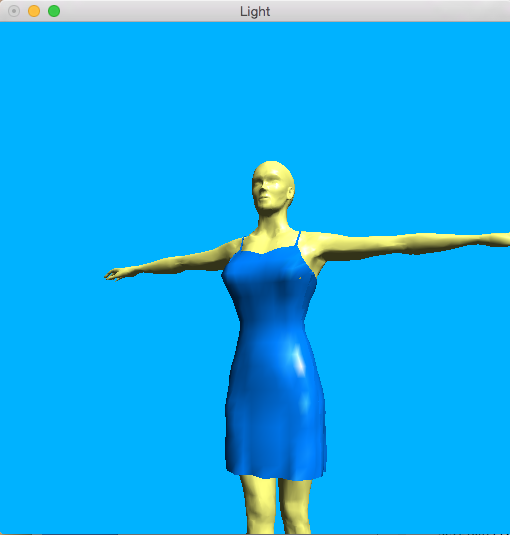
\includegraphics[height=10cm]{OGL_light/meshSmoothSurfaces.png}
    \caption{메시의 면을 그린 결과 (정점 단위로 법선 계산)}
    \label{fig:OGL_light:meshSmoothSurfaces}
\end{figure}

빛의 반사와 관련된 내용들에 대한 깊이 있는 이해를 위해서는 \cite{akenine2011real,pharr2004physically} 등을 참고하라.